\section{The importance of reductions}
A reduction in terms of parallel programming is an operation, where a large dataset of entries (e.g. numbers) is reducted to one entry.
The simplest example is the sum of a set of numbers and will be used for the rest of this work.
More generally are reduction is defined by an operation \( \circ: X \times X \rightarrow X \) on two entries with the following properties:
\begin{align}
    a \circ b &= b \circ a \ \ \mathrm{(commutativity)}, \\
    a \circ (b \circ c) &= (a \circ b) \circ c \ \ \mathrm{(associativity)}.
\end{align}
This guarantees that the result is (mathematically) independent of the order in which the elements are reduced.
Note, that these properties do not ensure numerical stablility.

The reduction operation, first and foremost the sum, plays a crucial role in all of numerics.
Simple linear algebra operations like the scalar product or the matrix multiplication already include a reduction:
The entries of two vectors are multiplied element wise and the summed up.
In machine learning, reductions are present as a key step in feed-forward networks:
Again all the values of the node one layer below are multiplied by weights elementwise and the summed up to calculated the value of a singular node above.
Reductions are a very basic and fundamental operation and, therefore, an efficient implementation is required. 

\section{The tree reduction algorithm}
\begin{figure}
    \centering
    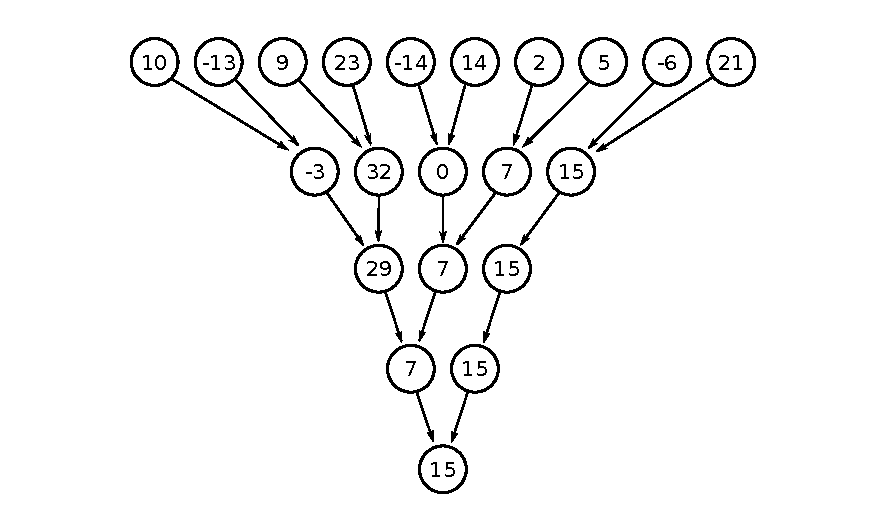
\includegraphics{tree_reduction.pdf}
    \caption{
        Example of a tree reduction of ten elements.
        Note how there is a leftover after the second reduction.
        These are usually handled by zeropadding (i.e. adding zeros) after each step to make the number of elements divisible by 2.
    }
\end{figure}
The most efficient algorithm is heavily dependent on the underlying hardware.
For example, a node network with a lot of parallelisation overhead and a complicated communication topology might use a ring algorithm ("add value and pass to next").
In this work the focus is on single GPU reductions.
Here, the tree reduction approach is the most successful.
All available threads are called to reduce two entries to one in parallel, effectively halfing the size of the dataset in one step.
This is repeated until only one entry remains.

\section{Naive implementation with CUDA}
For a better understanding of the framework of CUDA and tree reduction algorithm an unoptimized code is presented which implements the algorithm for the case of addition of signed 32-bit integers. 
Note, that even though this is unoptimized GPU code, it runs magnitudes faster than on a CPU (exact speedup depending on the problem size and the available hardware).

When approaching a problem using CUDA the big challenge is to map the for-loop that one wants to parallelize to blocks and CUDA-threads. 
Often, the best starting point is to write serial CPU code to get a feeling for the problem and to have a working solution to test the optimized solutions against later.
In this case, we will first implement a serial tree reduction in C and port this code to CUDA in a second step.

\subsection{Serial tree reduction on a CPU}
Our starting point is an integer array \texttt{h\_in}.
The \texttt{h\_} denotes data stored on the host (CPU RAM), which is a useful convention, since CUDA does not distinguish between pointers to host and device memory.
For simplicity, we assume that the size of the array is a power of two.
If this is not the case, one could simply zeropad the data and would still be able to use the code.

Lets write a function \texttt{reduce} that executes the tree reduction.
This function takes an input array \texttt{h\_in}, performs the reduction and writes the result to an output \texttt{h\_out}. 
We need two for-loops:
One to iterate over the step of the reduction (vertically in fig. \ref{fig_tree_reduction}) and one to iterate over the (remaining) data set (horizontally). 
A temporary array is used to do the reduction on, so the input array stays untouched.

\lstinputlisting[language=C]{code/host_reduce.c}

The inner loop of this implementation could be parallelised easily, since each step of the inner loop is independent.
This means, however, that with each step of the outer loop all threads are created and destroyed, which creates a large parallelisation overhead.
In general and independent of CPU or GPU, one should always aim to parallelize the outermost loop.
Here, the outer loop cannot be parallelized, since each step is dependent on the result of the step before.
To fix this, one can swap the two loops.
While this requires slightly more code, it greatly simplifies all examples in the following.
The rewritten function looks like this:

\lstinputlisting[language=C]{code/host_reduce_swapped_loops.c}

Note that an additional if-statement is required.
This is a much better basis for parallelisation, since now the outer loop can be parallelised.
However, one needs to be very careful as this is now prone to a race-condition.

It should be noted, that there are much faster ways to implement a reduction algorithm as a single-thread CPU application.
This code has been written with the intent of parallelisation on a GPU and serves solely this purpose.
